\documentclass[paper=A4,pagesize=auto,12pt,headinclude=true,footinclude=true,BCOR=0mm,DIV=calc]{scrartcl}

\usepackage[utf8]{inputenc}
\usepackage{amsmath}
\usepackage[T1]{fontenc}
\usepackage{lmodern}
\usepackage[ngerman]{babel}
\usepackage[hidelinks]{hyperref}
\usepackage{setspace}
\usepackage[left=25mm, right=25mm, top=25mm, bottom=25mm]{geometry}
\usepackage[backend=biber, style=ieee, citestyle=ieee]{biblatex}
\usepackage[table]{xcolor}
\usepackage{graphicx}
\usepackage{wrapfig}
\usepackage{lipsum}
\usepackage[nottoc,numbib]{tocbibind}
\usepackage{attachfile}
\onehalfspacing

\bibliography{forschungsbericht}

%opening
\title{Auswirkungen eines Hintergrundes auf die Identifikation von Objekten in Bildern mithilfe eines Convolutional Neural Network}
\author{Alexandra Zarkh, Sui Yin Zhang,\\ Lennart Leggewie und Alexander Schallenberg}

\makeatletter
\def\@maketitle{%
	\newpage
	\null
	\vskip 2em%
	\begin{center}%
		\let \footnote \thanks
		{\Huge \textbf{\@title} \par}%
		\vskip 3em%
		{\large
			\lineskip .5em%
			\begin{tabular}[t]{c}%
				\@author
			\end{tabular}\par}%
		\vskip 2em%
		{\large Hochschule Bonn-Rhein-Sieg, Fachbereich Informatik, D-53757\par}%
		\vskip 2em%
		{\large \@date}%
	\end{center}%
	\par
	\vskip 1.5em}
\makeatother


\setlength{\arrayrulewidth}{0.3mm}
\setlength{\tabcolsep}{10pt}

\newcommand{\sectionspace}{
	\vspace{0.5cm}
}

\newcommand*\justify{%
	\fontdimen2\font=0.4em% interword space
	\fontdimen3\font=0.2em% interword stretch
	\fontdimen4\font=0.1em% interword shrink
	\fontdimen7\font=0.1em% extra space
	\hyphenchar\font=`\-% allowing hyphenation
}

\renewcommand{\texttt}[1]{%
	\begingroup
	\ttfamily
	\begingroup\lccode`~=`/\lowercase{\endgroup\def~}{/\discretionary{}{}{}}%
	\begingroup\lccode`~=`[\lowercase{\endgroup\def~}{[\discretionary{}{}{}}%
	\begingroup\lccode`~=`.\lowercase{\endgroup\def~}{.\discretionary{}{}{}}%
	\begingroup\lccode`~=`(\lowercase{\endgroup\def~}{(\discretionary{}{}{}}%
	\catcode`/=\active\catcode`[=\active\catcode`.=\active\catcode`(=\active
	\justify\scantokens{#1\noexpand}%
	\endgroup
}

\renewcommand{\listoffigures}{\begingroup
	\tocsection
	\tocfile{\listfigurename}{lof}
	\endgroup}

\renewcommand{\listoftables}{\begingroup
	\tocsection
	\tocfile{\listtablename}{lot}
	\endgroup}

\begin{document}

\begin{titlepage}
	\maketitle
\end{titlepage}

\tableofcontents
\newpage


\section{Zusammenfassung}\label{sec:Zusammenfassung}
In diesem Forschungsbericht werden Auswirkungen eines Hintergrundes auf die Erkennung und Identifikation von Objekten in Bildern mithilfe eines sogenannten Convolutional Neural Network vorgestellt und diskutiert. Dies geschieht anhand des Beispiels der Erkennung und Identifikation von Verkehrszeichen auf Straßen.
Im ersten Teil des Textes wird die verwendete Literatur, die Theorie und die Fragestellung präsentiert. Anschließend folgen die Methoden, die zur Klärung der Fragestellung beitragen. Unter anderem wird hier erklärt, was ein Convolutional Neural Network ist und wie es hier implementiert wurde. Dort werden im Detail dann die Java-Dateien und deren Methoden sowie Attribute vorgestellt. Der letzte Teil des Abschnitts Methoden präsentiert dann die durchgeführten Test.
Zum Schluss werden die Ergebnisse aufgeführt und zusammengefasst. Daraufhin wird die Fragestellung des Berichts nochmal aufgegriffen und diskutiert. In den letzten beiden Abschnitten findet man sowohl die Verzeichnisse als auch den Anhang.

\sectionspace
\section{Einleitung}\label{sec:Einleitung} %Alexi
Die Gesichtserkennung am Smartphone ermöglicht das Entsperren eines Gerätes und auf verschiedenen Applikationen die Nutzung von Filtern, die das Gesicht und die Umgebung erkennen und entweder die Umgebung oder bestimmte Eigenschaften und Merkmale in Gesichtern selber verändern.
Das Autofahren wird immer einfacher und komfortabler für die Person am Steuer und das hat man unter anderem der Verkehrszeichen- und Fahrbahnlinienerkennung zu verdanken. Jetzt stellt sich die Frage: wie funktioniert das? Die Antwort ist Computer Vision. Computer Vision kann durch verschiedene Arten umgesetzt werden. Eine davon funktioniert mit künstlichen neuronalen Netzen. Dieses wird dann Convolutional Neural Network (kurz CNN oder ConvNet) genannt.

\subsection{Verwendete Literatur}\label{sec:VerwendeteLiteratur}
Grundlage des Convolutional Neural Network sind die Inhalte des Projektberichts \cite{projektbericht}. Außerdem bietet das Kapitel neun aus \citetitle{script} von \citeauthor{script} \cite{script} einige grundlegende Informationen der \textit{Computer Vision} verwendet. Der Theorie bzw. des Aufbaus des CNN dienen die Artikel \citetitle{cnn1} von \citeauthor{cnn1} \cite{cnn1} und \citetitle{cnn2} von \citeauthor{cnn2} \cite{cnn2}. Des Weiteren stammen einige kritische Aspekte der Diskussion aus \citetitle{discuss1} von \citeauthor{discuss1} \cite{discuss1}. 

\subsection{Theorie}\label{sec:Theorie} %Alexi
Computer Vision kann durch verschiedene Arten umgesetzt werden. Eine davon funktioniert mit künstlichen neuronalen Netzen. Etwas fortgeschrittener als ein knN ist in Bezug auf Bilderverarbeitung das Convolutional Neural Network (kurz CNN oder ConvNet). \cite{script}\\
Ein Auto kann mithilfe dessen durch ein Video oder ein Bild einer eingebauten Kamera beispielsweise Verkehrszeichen erkennen und auf sie reagieren. Dazu muss in diesem Video oder Bild zunächst ein Verkehrszeichen erkannt werden, es muss identifiziert werden, um welches Verkehrszeichen es sich handelt und es muss reagiert werden. Diese Erkennung und Identifikation ist Aufgabe eines solchen Convolutional Neural Network.

\subsection{Fragestellung}
Die Leitfrage ist nun: Welche Auswirkungen hat ein Hintergrund eines Bildes auf die Kosten der Kalkulation eines Convolutional Neural Network (CNN), welches ein Objekt im Vordergrund des Bildes erkennen und identifizieren soll?

\sectionspace
\section{Methoden}\label{sec:Methoden}
Die Fragestellung wird im Folgenden am Beispiel von acht Verkehrszeichen geklärt.

\subsection{Convolutional Neural Networks}\label{subsec:CNN} %Lennart
Ein Convolution Neural Network, ist ein Deep-Learning-Algorithmus, der ein Bild aufnimmt, verschiedenen Objekten im Bild eine Bedeutung zuweist und diese Objekte voneinander unterscheiden kann \cite{cnn1}. Das Convolutional Neural Network ist ein mathematisches Konstrukt das normalerweise aus Schichten oder Bausteinen besteht. Die ersten beiden Schichten, Convolution und Pooling-Schicht, extrahieren bestimmte Merkmale aus einem Bild, während die dritte Schicht, vollständig verknüpfte Schicht, die extrahierten Merkmale in die endgültige Ausgabe umsetzt. Eine typische Architektur besteht aus Wiederholungen eines Stapels von mehreren Convolution-Schichten und einer Pooling-Schicht gefolgt von mehreren vollständig verknüpften Schichten. Der Vorgang, bei dem die Eingabedaten durch diese Schichten in Ausgabedaten umgewandelt werden, wird als Vorwärtspropagation bezeichnet. Die in diesem Abschnitt erläuterten Convolution und Pooling-Operationen beziehen sich jedoch auf ein 2D-CNN, ähnliche Operationen können aber auch für 3D-CNN durchgeführt werden. \cite{cnn2}

\subsubsection{Convolution}
Convolution (im CNN auch Convolutional-Schicht) ist eine lineare Operation, die für die Merkmalsextraktion verwendet wird. Um bestimmte Merkmale zu extrahieren wird ein Array, der sogenannte Kernel, auf das Eingabe-Bild, das auch zu einem Array umgewandelt wurde, namens Kernel, angewendet.\\
Ein elementweises Produkt zwischen jedem Element des Kernels und dem Eingabetensor wird an jeder Stelle des Tensors kalkuliert und summiert, um den Ausgabewert an der zugehörigen Stelle des Ausgabetensors, einer so genannten Merkmalskarte, zu erhalten. Dieses Verfahren wird unter Anwendung mehrerer Kernel wiederholt, um eine beliebige Anzahl von Merkmalskarten zu erzeugen, die jeweils verschiedene Merkmale des Eingabetensors darstellen.\\
\begin{wrapfigure}{r}{0.5\textwidth}
	\centering
	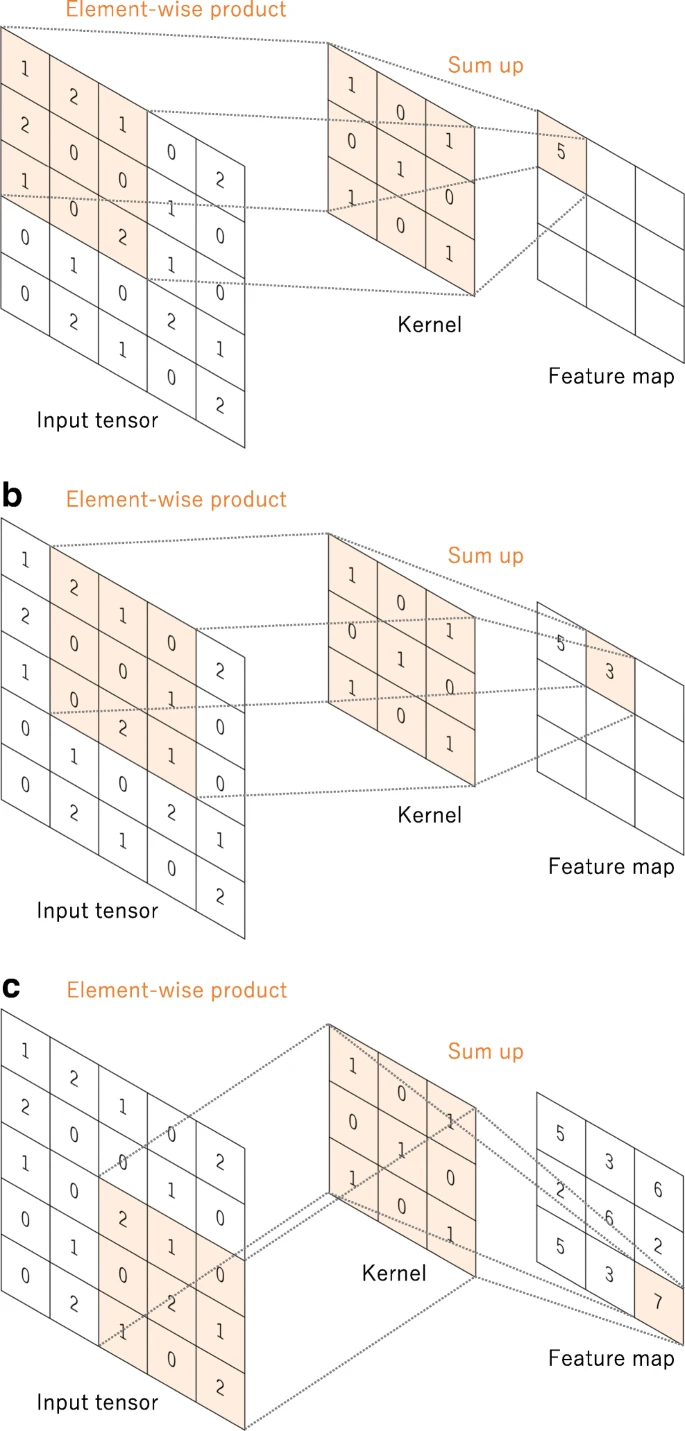
\includegraphics[width=6cm]{"images/cnn.png"}
	\caption{Benutzung des Kernels \cite{cnn2}}
	\label{useofkernel}
\end{wrapfigure}
Die hier beschriebene Convolution-Operation lässt nicht zu, dass die Mitte eines Kernels das äußerste Element des Eingabetensors überdeckt, und verringert somit die Höhe und Breite der Merkmalskarte. Das Auffüllen mit Nullen ist eine Technik zu Lösung dieses Problems, bei der Zeilen und Spalten mit Nullen auf jeder Seite des Eingabetensors angefügt werden, so dass das Zentrum eines Kernels auf das äußerste Element passt und die gleiche Dimension in der Ebene durch die Convolution-Operation beibehalten wird. Der Abstand zwischen zwei aufeinanderfolgenden Kernelpositionen wird als Stride bezeichnet, der auch die Convolution-Operation definiert. Üblicherweise wird ein Stride der Größe 1 gewählt, jedoch wenn man ein Downsampling  der Merkmalskarten erreichen möchte, wird ein Stride größer als 1 verwendet.

\subsubsection{Pooling-Schicht}
Eine Pooling-Schicht bietet eine klassische Downsampling-Operation, die die Dimensionalität der Merkmalskarten in der Ebene reduziert, um eine Übersetzungsinvarianz gegenüber kleinen Verschiebungen und Verzerrungen einzuführen und die Anzahl der nachfolgenden lernbaren Parameter zu verringern. Es ist hervorzuheben, dass es in keiner der Pooling-Schichten einen lernbaren Parameter gibt, während Filtergröße, Stride und Padding Hyperparameter bei Pooling-Operationen sind, ähnlich wie bei Convolution-Operationen. \cite{cnn2}

\subsubsection{Max Pooling}
Die gängigste Form der Pooling-Operation ist das Max-Pooling, bei dem aus den eingegebenen Merkmalskarten Felder extrahiert werden, der maximale Wert in jedem Feld ausgegeben und alle anderen Werte verworfen werden. Üblicherweise wird ein Filter der Größe 2 x 2 mit einem Stride von 2 verwendet. Dadurch wird die In-Plane-Dimension der Merkmalskarte um den Faktor 2 verkleinert. \cite{cnn2}

\subsubsection{Global Average Pooling}
Eine weitere erwähnenswerte Pooling-Operation ist das Global Average Pooling, dass eine extreme Art des Downsamplings durchführt. Hierbei wird eine Merkmalskarte mit einer Größe von Höhe x Breite in ein 1 x 1 Array verkleinert, indem der Durchschnitt aller Elemente in jeder Merkmalskarte gebildet wird, während die Tiefe der Merkmalskarte erhalten bleibt. In der Regel wird dieser Vorgang nur einmal vor den vollständig verknüpften Schichten durchgeführt. Der erste Vorteil des Global Average Pooling’s ist, dass die Anzahl der lernbaren Parameter reduziert wird und der zweite Vorteil ist, dass das Convolutional Neural Network Eingaben variabler Größe akzeptieren kann. \cite{cnn2}

\subsubsection{Vollständig Verknüpfte Schicht}
Die Ausgangsmerkmalskarten der letzten Convolution oder Pooling-Schicht werden in der Regel abgeflacht, das heißt in ein eindimensionales Zahlenfeld umgewandelt und mit einer
\begin{wrapfigure}{r}{0.5\textwidth}
	\centering
	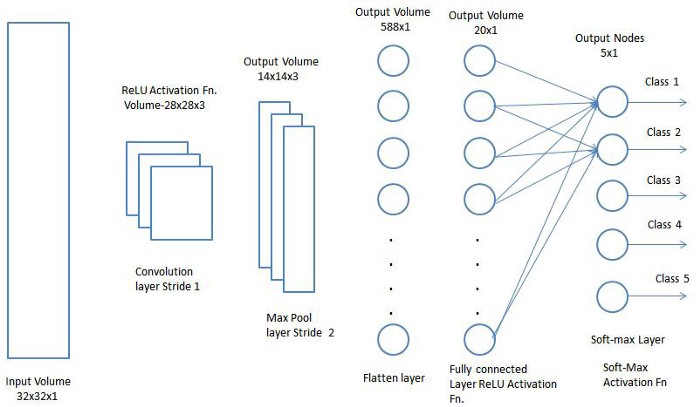
\includegraphics[width=6cm]{"images/vollst_verk_schicht.png"}
	\caption{Benutzung des Kernels \cite{cnn1}}
	\label{polyconnected}
\end{wrapfigure}
oder mehreren vollständig verknüpften Schichten, auch als dichte Schichten bekannt, verbunden, in der jeder Eingang mit jedem Ausgang durch ein lernbares Gewicht verbunden ist. Sobald die von den Convolution-Schichten extrahierten und von den Pooling-Schichten heruntergestuften Merkmale erstellt sind, werden sie von einer Untergruppe vollständig verknüpften Schichten auf die endgültigen Ausgaben des Netzes abgebildet, zum Beispiel die Wahrscheinlichkeiten für jede Klasse bei Klassifizierungsaufgaben. Die letzte vollständig verknüpfte Schicht hat in der Regel die gleiche Anzahl von Ausgangsknoten wie die Anzahl der Klassen. \cite{cnn2}


\subsection{Implementierung} %Sui Yin
Die Implementierung in Java 17 besteht aus den vier neuen Klassen \texttt{ImageAdapter}, \texttt{ConvNet}, \texttt{RoadSignLabel}, \texttt{RoadSignTest} und einem Record \texttt{TrainData}. Zum Testen wird eine weitere Klasse und ein Enum verwendet. Diese vier neuen Klassen, das Record sowie die Testdateien werden im Folgenden Absätzen erklärt.

\subsubsection{ConvNet} %Alex
Die Klasse \texttt{ConvNet} soll ein Convolutional Neural Network darstellen und erbt daher von der im Projektbericht \cite{projektbericht} unter Abschnitt 2 genannten Klasse \texttt{Network}, was jener die gleichen Eigenschaften verleiht. Des Weiteren besitzt sie eine \texttt{java.util.ArrayList} vom Generic-Typ \texttt{TrainData} und einen \texttt{ImageAdapter} als private konstante Attribute. Erstere dient dem Speichern von Trainingsdatensätzen, die dann mit dem Aufrufen der überladenen Methode \texttt{train(double, int)} benutzt werden. Diese ruft die originale Instanz-Methode \texttt{train(double[][], double[][], double, int)} der Klasse \texttt{Network} mit den Daten aus der \texttt{ArrayList} auf.
Außerdem bietet die Klasse \texttt{ConvNet} die Instanz-Methoden \texttt{addTrainData(String, int[])} und \texttt{addTrainData(String, int[], boolean)} um dieser Trainingsdatensätze hinzuzufügen. Diese nehmen einen Dateinamen von einem Bild und einen ganzzahligen Zielvektor. Zweitere nimmt zusätzlich einen Wahrheitswert, der bestimmt, ob das Bild vor dem Benutzen bearbeitet werden soll. Erstere Methode ruft die Zweite mit dem Wahrheitswert \texttt{false} auf. Zwei private nicht-statische Hilfsmethoden \texttt{getImages()} und \texttt{getTargets()} dienen der besseren Handhabung der \texttt{ArrayList}.\\
Die Klasse erstellt durch den Konstruktor \texttt{ConvNet(String, int, int, int, int[])} (Pfad zum Ordner mit den Bildern, gewünschte Bildweite, -höhe, Anzahl der Output-Neuronen, Anzahl der Hiddenlayers und deren Neuronen) von ihr abgeleitete Objekte.

\subsubsection{ImageAdapter} %Sui Yin
Der \texttt{ImageAdapter} ist dafür da, um das Bild zu laden und skalieren.
Die Klasse besteht aus sechs Methoden und einem Konstruktor. 
Im Konstruktor \texttt{ImageAdapter(String, int, int)} werden Pfad zu den Bildern, gewünschte Bildhöhe sowie -breite als Parameter übergeben, mit denen dann die jeweiligen Skalierungswerte für das jeweilige Bild initialisiert werden.
Die Methode \texttt{loadImage(String)} lädt das \texttt{java.awt.image.BufferedImage} mit dem übergebenen Namen und gibt es zurück.
Falls es keine Datei mit diesem Namen gibt oder diese keine Bilddatei ist, wird eine \justify{\texttt{IllegalArgumentException}} eine geworfen.
Als nächstes geht die Methode \texttt{getRGBs(BufferedImage)} alle Pixel durch und gibt deren hexadezimale RGB-Werte als Matrix für das jeweilige Bild zurück.
Die Methode \texttt{squareImage(BufferedImage)} ist dafür da, um das Bild quadratisch zuzuschneiden. 
\texttt{scaleImage(BufferedImage)} skaliert ein Bild mit einer beliebigen Höhe oder Breite.
Um ein \texttt{java.awt.image.Image} in ein \texttt{java.awt.image.BufferedImage} konvertieren, wird die Methode \texttt{convertToBufferedImage(Image)} benutzt.
In der einzigen öffentlichen Methode des \texttt{ImageAdapter}s \texttt{getImageRGBs(String, boolean)} wird mit den genannten Methoden und mithilfe eines übergebenen Dateinamens und eines Wahrheitswerts ein eindimensionales ganzzahliges Array mit allen RGB-Werten per \textit{row-major order}
\begin{equation}
	\scalebox{1.3}{$m_{ij} \rightarrow a_{64\cdot i + j}$}
\end{equation}
des aus dem Dateinamen resultierenden Bildes zurückgegeben. Der Wahrheitswert bestimmt, ob das Bild, welches geladen wird, zugeschnitten und skaliert werden soll, oder nicht.

\subsubsection{TrainData}
Das Record \texttt{TrainData(int[], int[])} besitzt einen Vektor mit den RGB-Werten eines Bildes und einen Zielvektor. Außerdem hat es zwei Instanz-Methoden \texttt{getImageAs-DoubleArray()} und \texttt{getTargetAsDoubleArray()}, welche die jeweiligen ganzzahligen Vektoren als Gleitkommazahl-Vektoren zurückgibt, und eine private nicht-statische Hilfsmethode \texttt{getIntAsDoubleArray(int[])}.

\subsubsection{Test-Dateien} %Alex
Für das Testen wurden ein Enum \texttt{RoadSignLabel} und eine Klasse \texttt{RoadSignTest} implementiert. Das Enum zählt die möglichen Ergebnisse des Netzes auf, indiziert sie und kann den jeweils richtigen Zielvektor durch die Instanz-Methode \texttt{getTarget()} zurückgeben. In der Klasse befindet sich die für die Forschungsfrage relevante Main-Methode des Programms. Diese ruft eine private statische Methode \texttt{test()} in der selben Klasse auf. In dieser wird ein \texttt{ConvNet} deklariert und initialisiert, mit Datensätzen bestückt und trainiert. Dabei werden einige hilfreiche Ausgaben gemacht.

\subsection{Tests}
\rowcolors{2}{white}{lightgray}
Für das Testen wurden  43 Bilder mit Verkehrszeichen gesammelt, einige gut erkennbar, andere schwieriger. Diese Originalbilder sind dann zu 128x128px-Bildern konvertiert worden, um einen Netzeingabevektor konstanter Größe gewährleisten zu können. 
Die konvertierten Bilder seien im folgenden der Datensatz $b$. Dieser und ein daraus resultierender Datensatz $b'$, wobei der Hintergrund durch einen weißen (0xFFFFFF) Hintergrund ersetzt wurde, sind nun zum Testen verwendet worden. So ist um ein direkter Vergleich von Datensatz $b$ ``mit Hintergründen'' und Datensatz $b'$ ``ohne Hintergründe'' möglich. Die Bilder sind in acht Gruppen aufgeteilt, zeigen also acht unterschiedliche Verkehrszeichentypen: \textit{Andreaskreuz}, \textit{Fußgängerüberweg}, \textit{Gefahrenstelle}, \textit{Vorfahrt gewähren}, \textit{Vorfahrtstraße}, \textit{Verbot der Einfahrt}, \textit{Fußgängerweg} und \textit{Stopp}. Fast alle Bilder sind genau einer Gruppe zugeordnet. Ausnahmen sind zwei Bilder, die jeweils den beiden Gruppen \textit{Fußgängerüberweg} und \textit{Vorfahrt gewähren} zugeordnet sind. 
\begin{wraptable}{l}{0.5\textwidth} %l, r, c, i, o
	\centering
	\begin{tabular}{|c|c|}
		\hline
		\multicolumn{2}{|c|}{\textbf{Gruppen der Bilder}}\\ \hline
		\textbf{Gruppe} & \textbf{Anzahl} \\ \hline \hline
		Andreaskreuz & 5 \\ \hline
		Fußgängerüberweg & 6 \\ \hline
		Gefahrenstelle & 2 \\ \hline
		Vorfahrt gewähren & 6 \\ \hline
		Vorfahrtstraße & 6 \\ \hline
		Verbot der Einfahrt & 8 \\ \hline
		Fußgängerweg & 8 \\ \hline
		Stopp & 4 \\ \hline
	\end{tabular}
	\caption{Anzahl der Bilder pro Gruppe}
	\label{imagegroups}
\end{wraptable}
Das Convolutional Neural Network, welches zum Testen verwendet wird, ist auf einen 16384-dimensionalen Eingabevektor konfiguriert. Es besitzt vier versteckte Schichten, wobei die Erste und Zweite jeweils 64 Neuronen und die Dritte und Vierte 32 Neuronen haben. Die Ausgabeschicht besteht aus acht Neuronen. Der acht-dimensionale Ausgabevektor klassifiziert das jeweilige/die jeweiligen Verkehrszeichen in dem eingegebenen Bild.\\
Nun wurde sich angeschaut wie sich die Kosten nach jeder Epoche des Lernens des CNN abhängig vom verwendeten Datensatz verändern. Dazu wurde durch wiederholtes Anpassen eine Lernrate von 0.1111 gewählt. Das Training ist 1000 mal wiederholt worden, besteht also aus 1000 Epochen. Die Gewichtungen wurden zufällig mit Werten im Intervall [-0.5, 0.5) initialisiert. Das Convolutional Neural Network wurde nacheinander mit beiden Datensätzen trainiert. Die Ausgangsgewichtungen waren dabei gleich.\\
Dieses Training wurde mehrfach wiederholt, um Aussagekraft des Tests zu erhöhen.
%\vspace{2em}
%\begin{center}
%	\begin{tabular}{|c|c|c|c|c|c|}
%		\hline
%		\multicolumn{6}{|c|}{\textbf{Anzahl Neuronen im CNN}}\\ \hline \hline
%		\textbf{Input} & \textbf{Hidden 1} & \textbf{Hidden 2} & \textbf{Hidden 3} & %\textbf{Hidden 4} & \textbf{Output}\\ \hline
%		16384 & 64 & 64 & 32 & 32 & 8\\ \hline
%	\end{tabular}
%	\vspace{2em}
%	\begin{tabular}{|c|c|}
%		\hline
%		\multicolumn{2}{|c|}{\textbf{Bildgröße}}\\ \hline \hline
%		\textbf{Höhe} & \textbf{Breite}\\ \hline
%		128 & 128\\ \hline
%	\end{tabular}
%	\vspace{2em}
%	\begin{tabular}{|c|c|}
%		\hline
%		\multicolumn{2}{|c|}{\textbf{Training}}\\ \hline \hline
%		\textbf{Lernrate} & \textbf{Wiederholungen}\\ \hline
%		0.1111 & 1000\\ \hline
%	\end{tabular}
%\end{center}


\newpage
\sectionspace
\section{Ergebnisse}
Das Testen ergab, dass die Kosten bei beiden Datensätzen stetig fallen, also die Steigung der Kosten im gesamten Epochen-Intervall [1, 1000] negativ ist. Bei beiden sind die Kosten vor allem zwischen den ersten beiden Epochen sehr stark gesunken. 
\begin{wrapfigure}{c}{0.7\textwidth}
	\centering
	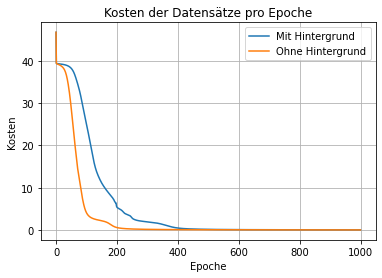
\includegraphics[width=10cm]{"images/test_plot.png"}
	\caption{Kosten der Datensätze pro Epoche}
	\label{testplot1}
\end{wrapfigure}
Danach ist die Steigung der Kosten für einige Epochen nahe 0, wird aber von Epoche zu Epoche kleiner. Darauf folgt ein annähernd exponentieller Verlauf. Während bei Datensatz $b$ im Epochen-Intervall [190, 260] kleinere Abweichungen einer Exponentialfunktion zu verzeichnen sind, worauf bis Epoche 420 eine größere Abweichung folgt, ist in Datensatz $b'$ nur eine größere Abweichung zu finden, wobei diese bereits im Intervall [100, 250] liegt. Die Kosten beider Datensätze nähern sich bis Epoche 1000 exponentiell der 0. Vergleicht man beide Verläufe, so sinken anfangs die Kosten von $b'$ ($C_{b'}$), also dem Datensatz ``ohne Hintergrund'' schneller als die Kosten von $b$ ($C_{b}$), also dem Datensatz ``mit Hintergrund''. Die Differenz $C_{b}-C_{b'}$ wird zwar nie 0, jedoch sinkt sie ebenfalls exponentiell, da $C_{b}$ und $C_{b'}$ beide exponentielle Verläufe aufweisen. \\
Wiederholt man das Testen mit verschiedenen Gewichtsmatrizen, so ergeben sich auch hier zu den beschriebenen Entwicklungen ähnliche Verläufe. \\
Welche Auswirkungen hat nun ein Hintergrund eines Bildes auf die Kosten der Kalkulation eines Convolutional Neural Network, welches ein Objekt im Vordergrund des Bildes erkennen und identifizieren soll? Den Tests ist zu entnehmen, dass der Hintergrund die Erkennung und Identifikation des Objektes, also in dem getesteten Beispiel des/der Verkehrszeichen, erschwert.



\sectionspace
\section{Diskussion}
Die Erschwerung der Erkennung und Identifikation der Verkehrszeichen durch den Hintergrund ist in mehreren Aspekten begründet.
Viele dieser Aspekte gehen nicht direkt vom Convolutional Neural Network selber aus, sondern von der Umgebung. Wie zum Beispiel Verkehrszeichen, die schwer zu erkennen sind, weil sie entweder schon sehr alt und dreckig sind oder zugeklebt wurden. Das erschwert dem CNN die Erkennung des Verkehrszeichens und kann zu Irrtümern führen, die dann im schlimmsten Fall einen Unfall verursachen können. 
Ein weiteres Problem könnte der Verkehrszeichenwald in der Stadt sein. Dann wird es für das Convolutional Neural Network schwerer, sich das gewollte Verkehrszeichen auszusuchen, da mittlerweile sehr viele Verkehrszeichen an einem Ort angebracht sind. Schwieriger wird es auch für das Convolutional Neural Network ein Verkehrszeichen zu erkennen, wenn der Hintergrund sehr farbig ist und den Farben des Verkehrszeichens ähnelt. Dann könnte es schwierig werden, das Bild zurecht zuschneiden und die Ränder des Verkehrszeichens zu erkennen.  \cite{discuss1}\\
Andererseits kann man den Tests entnehmen, dass durch ausreichend Training mit ggf. komplexeren Netzen und/oder größeren Trainingsdatensätzen die Auswirkungen von Hintergründen minimiert werden können.

\subsection{Vor- \& Nachteile der gewählten Umsetzung}
Die Benutzung des Neuronalen Netzes aus dem Projektbericht \cite{projektbericht} hat den Vorteil, das dort schon diverse Perfektionierungsüberlegungen getätigt und teilweise umgesetzt wurden. Das benutzte Netz ist also schon recht performant. Außerdem bewirkt dies zusammen mit der Auslagerung des Handhaben der Bilder in den \texttt{ImageAdapter}s und des ``Test-Frameworks'' übersichtlichen und nachvollziehbaren Java-Quellcode.\\
Leider ist die Programmiersprache Java durch einige Aspekte eher ungeeignet für eine Performace-orientierte Umsetzung eines künstlichen neuronalen Netzes bzw. eines Convolutional Neural Networks. Eine Alternative wäre, ein solches Netz in der Programiersprache Python zu implementieren, welche dafür bekannt ist, in ihr künstliche neuronale Netze umzusetzen. Die gewählte Umsetzung ist außerdem zu jeglichen Visualisierungen zum Beispiel des Trainings oder der Ergebnisse des Training ungeeignet. 

\newpage
\sectionspace
\section{GitHub}
Unser Projekt inklusive der Datensätze, der Originalbilder und deren Quellen (nur von den nicht Selbstaufgenommenen) und dieses Forschungsberichts steht auf \textbf{GitHub} (\hyperref{https://github.com/Griszder/ProjektSeminar.git}{}{}{\textit{https://github.com/Griszder/ProjektSeminar.git}}) zur Verfügung.

\sectionspace
\section{Anteile am Gesamtprojekt}
Das Gesamtprojekt teilt sich in mehrere Teile. Während Herr Leggewie viel Aufwand in die Recherche und die Formulierung des Abschnittes \ref{subsec:CNN} steckte, befasste sich Frau Zarkh mit Einleitung und Theorie des Forschungsberichts. Frau Zhang und Herr Schallenberg teilten sich den Abschnitt 3.2 \textit{Implementierung}. Unterkapitel 3.3 ist zum großen Teil von Herrn Schallenberg verfasst. Die Originalbilder der Testdatensätze wurden von Frau Zhang herausgesucht bzw. fotografiert. Der Testdatensatz ``mit Hintergründen'' ist von Herrn Schallenberg angefertigt worden, den Testdatensatz ``ohne Hintergründe'' haben er, Frau Zarkh und Frau Zhang gemeinsam erstellt. Die Implementierung wurde von der ganzen Gruppe entwickelt und von Herrn Schallenberg getippt. Die Präsentation haben Frau Zarkh, Frau Zhang und Herr Leggewie erstellt.\\
Abschließend ist festzuhalten, dass alle Gruppenmitglieder in etwa gleich viel Aufwand in das Gesamtprojekt investiert haben.

\newpage
\printbibliography[heading=bibnumbered]

\sectionspace
\listoffigures
\sectionspace
\listoftables

\sectionspace
\section{Anhang}
\attachfile{attachments/projektbericht.pdf}{ Projektbericht}


\end{document}
